\documentclass[11pt]{article}
\usepackage{titlesec}
\usepackage{mhchem}
\usepackage{array}
\usepackage{graphicx}
\usepackage[bmargin=2cm, tmargin=2cm]{geometry}
\usepackage{fourier-orns}
\usepackage{tikz}
\usepackage{amsfonts}
\usepackage{amssymb}
\usepackage{amsmath}
\usepackage{physics}


\newcommand{\thedate}[1]{\hfill{\small\sc #1}}
\newcommand{\NB}{{\large\lefthand}\quad}
\newcommand{\cm}{cm\(^{-1}\) }
\renewcommand{\d}{\text{d}}
\mathchardef\Re="023C
\mathchardef\Im="023D
\let\oldRe\Re
\let\oldIm\Im
\renewcommand\Re[1]{\oldRe\mathfrak{e}\left\{#1\right\}}
\renewcommand\Im[1]{\oldIm\mathfrak{n}\left\{#1\right\}}
\titleformat{\section}[runin]{\sc\Large}{\S\thesection}{3ex}{}[]
\titleformat{\subsection}[runin]{\sc\large}{\S\thesubsection}{3ex}{}[]
\titleformat{\subsubsection}[runin]{}{\S\thesubsubsection}{1ex}{\bfseries}[.]

\newtheorem{defn}{Definition}[section]

\title{The Quantum World}
\date{}
\author{}
\begin{document}
\maketitle
\section{Fourier Analysis}\thedate{5/10/20 --- Week 2}
\subsection{Fourier Series}
    \begin{align*}
        f(t) &= \sum_{n=-\infty}^{+\infty} C_n e^{in\omega_0t}
    \end{align*}
    Where $\omega_0$ is the fundamental frequency, and $n\omega_0$ is the $n$th harmonic.
    The superposition of these waves gives us our final function. Do not panic about negative frequencies,
    it will all become clear later on.
    \begin{alignat*}{2}
        f(t) &= \cos(\omega_0t)\\
        &= \frac{1}{2}e^{i\omega_0t} +& \frac{1}{2}e^{-i\omega_0t}\\
        &n=1 & n=-1\\
        &C_1 = \frac{1}{2} &C_{-1} = \frac{1}{2}\\
        f(t) &= \frac{1}{2}e^{i\omega_0t} +& \frac{1}{2}e^{-i\omega_0t}\\
    \end{alignat*}
    Plotting this as a fourier spectrum. We have ommited the imaginary part (because there isn't one), however
    if there were we would simply plot the modulus squared.
    % \begin{figure}[h]
    %     \centering
    %     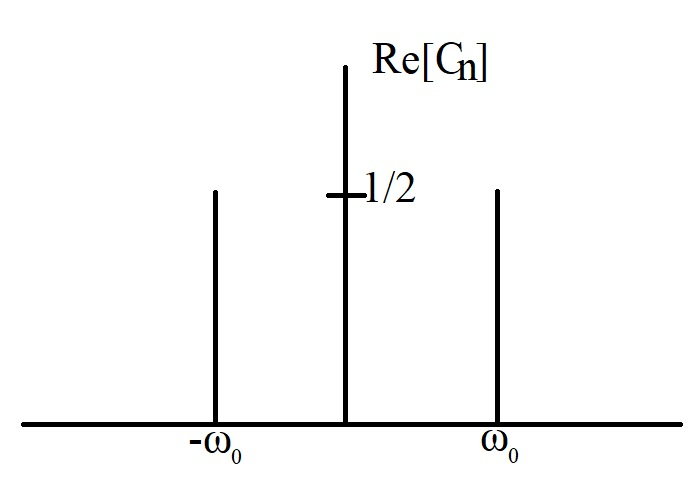
\includegraphics[width=10cm]{spec1.jpg}
    % \end{figure}

    \begin{center}
        \begin{tikzpicture}[x=4cm, y=4cm, thick]
            \draw (-1, 0) -- (1, 0);
            \draw (0, 0) -- (0, 1) node[anchor=mid west]{\(\Re{C_n}\)};
            \draw (0.7, 0) node[anchor=north]{\(\omega_0\)} -- (0.7, 0.5);
            \draw (-0.7, 0) node[anchor=north]{\(-\omega_0\)} -- (-0.7, 0.5);
            \draw (-0.05, 0.5) -- (0.05, 0.5) node[anchor=mid west]{\(\frac{1}{2}\)};
        \end{tikzpicture}
    \end{center}
        
    But how do we find $C_n$ for a general case?

    \begin{align*}
        C_n = \frac{1}{T} \int_{t_0}^{t_0 + T} f(t) e^{-in\omega_0 t}\ \d{t}\\
    \end{align*}

    Where T is the period. Just like frequency is the reciprocal of time, we can have reciprocal space.
    We have a \emph{spacial frequency}, $k$, that is related to the inverse of the period of a wave in space
    (its wavelength). We call this spacial frequency the \emph{wavenumber}. It is more the spacial equivalent
    of angular frequency.
    \begin{align*}
        k = \frac{2\pi}{\lambda}
    \end{align*}
    From the de Brogile relationship it is obvious that the momentum of a quantum particle is inversely related
    to its wavelength
    \begin{align*}
        p = \frac{h}{\lambda}\\
        p = \hbar k
    \end{align*}
    We can see how momentum and position are inversely related (k is the inverse of position.)

    \subsection{Fourier Transforms}
    Fourier series are only really useful for periodic functions. An aperiodic function is very useful for 
    things like wavepackets and 1D particles in boxes which do have a repeating pattern along the x-axis.
    
    We will have to use a Fourier transform, unlike a Fourier series, which is a discrete set of coefficients,
    \(c_n\), for a discrete set of frequencies, a Fourier transform is a continuous function. As we can see below
    when we increase the seperation between the pulses, \( T \to \infty\), more frequency components appear on
    the Fourier spectrum. This means that the separation between the components \(\Delta\omega\) gets smaller
    until it approaches d\(\omega\). This arises from the reciprocal nature of time and frequency, as the period
    increases it should be expected that frequency separtion is to  reduce. The same is true of position and wavenumber.

    \begin{center}
        \textbf{Wide in time, narrow in frequency}\\
        \textbf{Wide in position space, narrow in momentum space}
    \end{center}

    \begin{figure}[h]
        \centering
        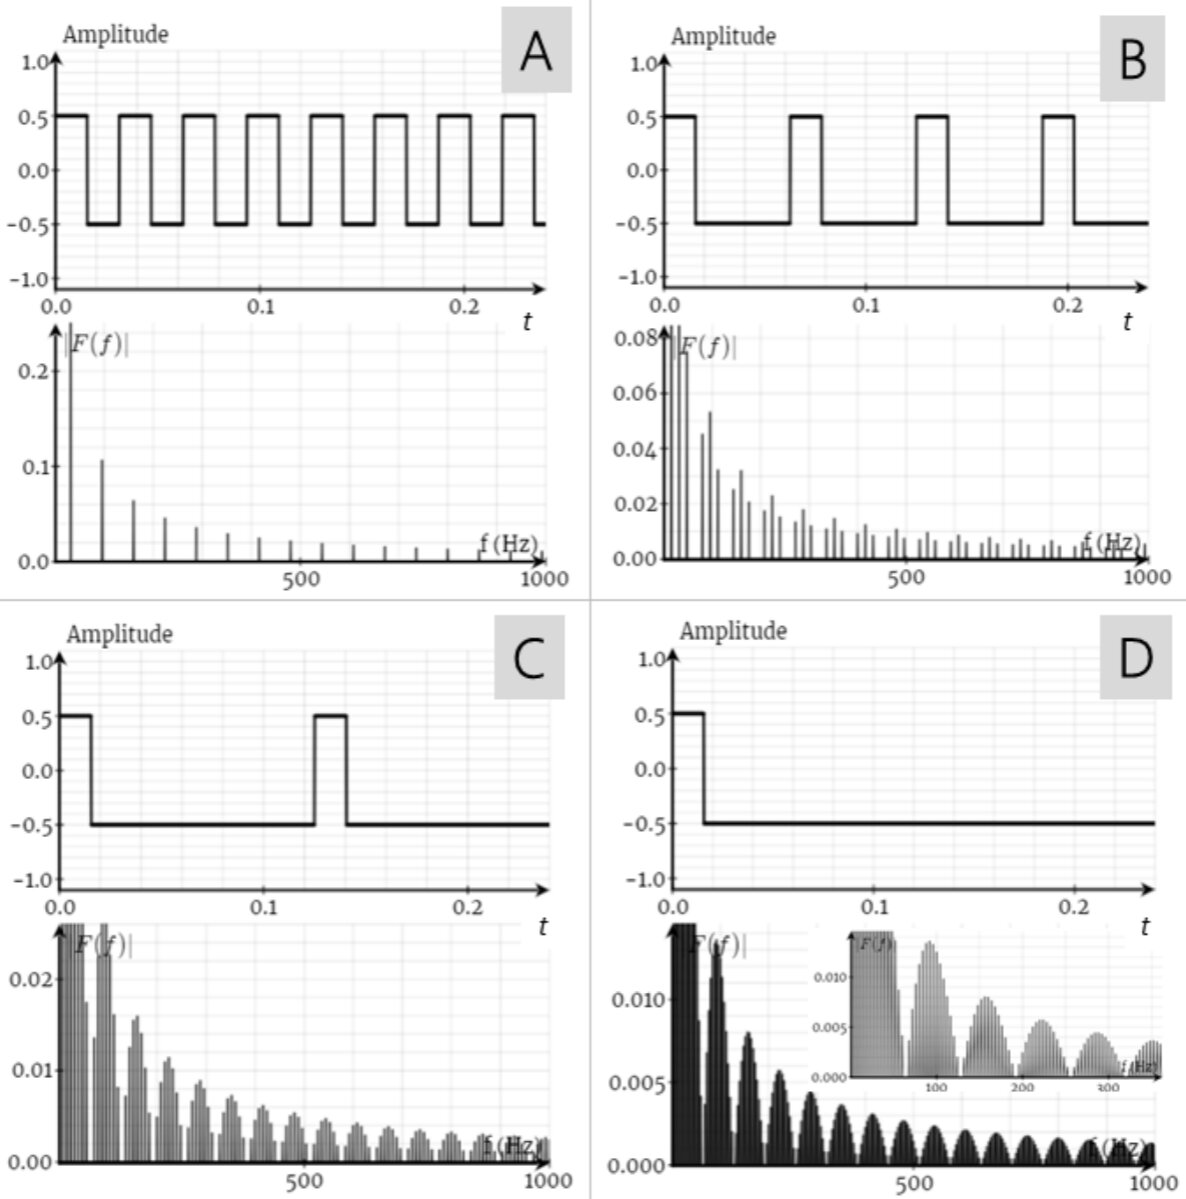
\includegraphics[width=8cm]{1.jpg}
        \caption{Increasing of T results in lowering of f separation}
    \end{figure}
    
    \begin{align*}
        F(\omega) = \frac{1}{\sqrt{2\pi}} \int_{-\infty}^{+\infty} f(t) e^{-i\omega t} dt\\
        F(k) = \frac{1}{\sqrt{2\pi}} \int_{-\infty}^{+\infty} f(x) e^{-ikx} dx
    \end{align*}

    As \(T \to \infty\) the frequency separation d\(\omega\) becomes infitesimally small, so the Fourier
    transformation is the \emph{integral} above, the spectrum becomes continuous. This transformations "translates" a function to its representation
    in terms of frequency. 

    \subsection{The Uncertainty Principle}
    The uncertainty principle arises not from a disturbance during measurment but because of the fundamental
    physics of waves. It happens at any scale, not just quantum. If we narrow a function of time its frequency
    must increase. 

    We can see this in a top-hat function, that is 0 everywhere except for a certain range of values \(2a\) wide
    where it is 1. It is thus an aperiodic function of a certain width, a pulse in time or a narrow region of space.

    \begin{figure}[h]
        \centering
        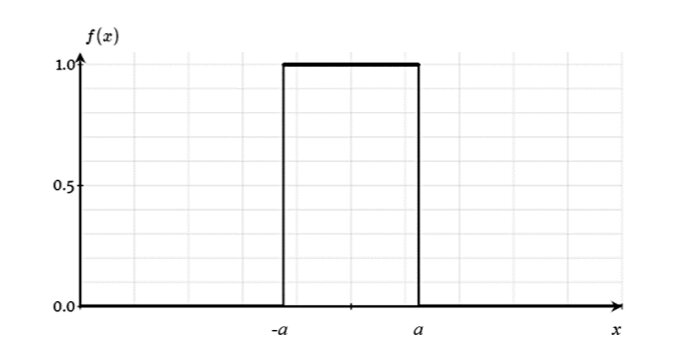
\includegraphics[width=8cm]{2.jpg}
        \caption{Top hat function of width 2a}
    \end{figure}

    This top hat function Fourier transforms into a sinc (\(\frac{\sin x}{x}\)) function.

    \begin{figure}[h]
        \centering
        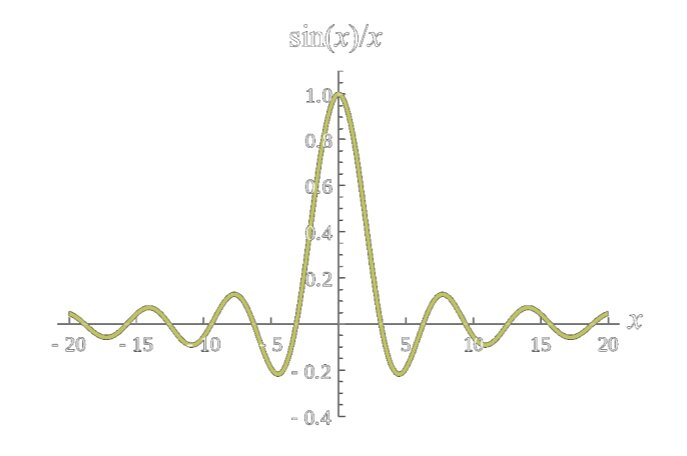
\includegraphics[width=8cm]{3.jpg}
        \caption{Sinc function}
    \end{figure}

    \begin{figure}[h]
        \centering
        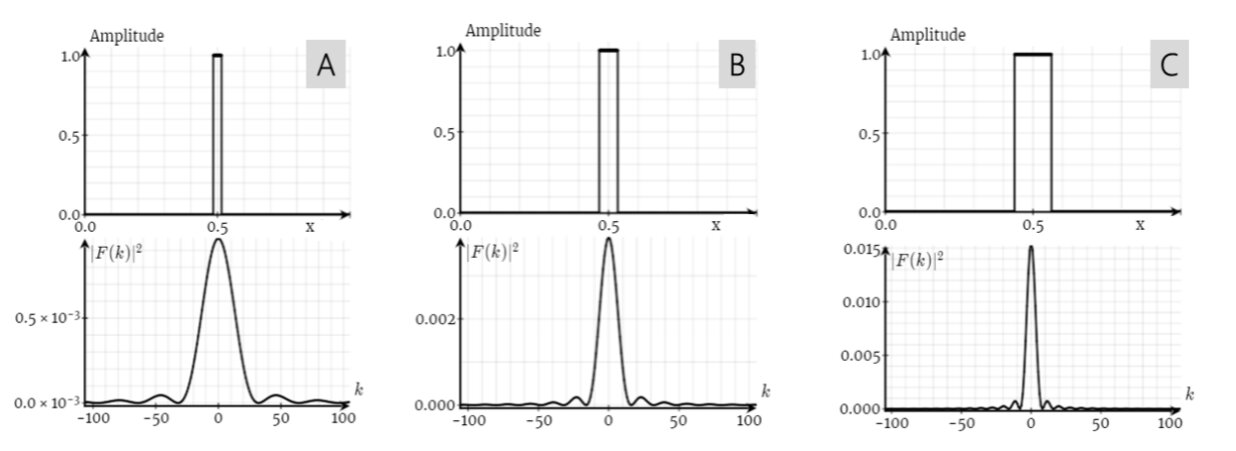
\includegraphics[width=8cm]{4.jpg}
        \caption{Sinc function}
    \end{figure}

    The relationship between position (real) space and momentum (reciprocal) space is shown well when examining
    the effect of narrowing the width of the top hat function on its Fourier transform. As the width increases
    the Fourier transform gets narrower.

    

\end{document}